\documentclass[hidelinks,oneside]{scrbook}			%
\usepackage[english]{babel}
\usepackage[pdftex]{graphicx} 	% Einbinden von Bildern
\usepackage{tabularx}
\usepackage{float}			%H in grafiken
\usepackage{amssymb}
\usepackage[left=2.5cm, right=2.5cm, bottom=2.5cm, top=2cm]{geometry}
\usepackage{verbatim}
\usepackage{lipsum}
\usepackage{booktabs} % for nicer tables
\usepackage{siunitx} % SI_UNITS https://www.dickimaw-books.com/latex/thesis/html/siunitx.html
\usepackage{amsmath}
\usepackage{braket} %bra-ket notation
\usepackage{hyperref}
\usepackage{epstopdf}
\usepackage{graphicx}
\usepackage{capt-of}
\usepackage{tikz}
\usepackage{algorithm}
\usepackage{algpseudocode}
\usepackage[font=small,labelfont=bf,labelsep=space]{caption}
\usepackage[caption=false,font=footnotesize]{subfig}

%%%%%%%%%%%%%%%%%%%%%%%%%%%%%%%%%%%%%%%%%%%%%%%%%%%%%%%%
% DOC FORMAT SETTINGS
\setlength\parindent{0pt}
\captionsetup{figurename=Fig.,	tablename=Tab.	}
%%%%%%%%%%%%%%%%%%%%%%%%%%%%%%%%%%%%%%%%%%%%%%%%%%%%%%%%
% TIKZ SETTINGS
\usetikzlibrary{shapes.geometric,
                calc, %for relative coord calculations
                decorations.pathmorphing, %for snake lines
                decorations.pathreplacing, %for braces
                shapes,
                arrows.meta, % for double arrow
                backgrounds,
                positioning} % for position along lines
%%%%%%%%%%%%%%%%%%%%%%%%%%%%%%%%%%%%%%%%%%%%%%%%%%%%%%%%
% Custom functions

\newcommand{\gtlt}{% greater than less than
{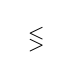
\begin{tikzpicture}%
\node[inner sep=0, outer sep=0] at (0,0) {$\scriptstyle <$};
\node[inner sep=0, outer sep=0] at (0,-0.15) {$\scriptstyle >$};
\end{tikzpicture}%
}}








%%%%%%%%%%%%%%%%%%%%%%%%%%%%%%%%%%%%%%%%%%%%%%%%%%%%%%%%
\begin{document}
\begin{titlepage}
\begin{center}
    \vspace*{15mm}
    
\includegraphics[width=100mm]{./graph/TU_Logo.pdf}
    
    \vspace{20mm}
    
    {\Large \textsc{Bachelor Thesis:}}
    
    \vspace{7mm}
    
    \rule{\textwidth}{0.4pt}\vspace{5mm}
    {\LARGE \textbf{Photoexcitations in a Quantum Dot - Benzene Heterostructure with non-local Coulomb Interactions}} \\[3mm]
    \rule{\textwidth}{0.4pt}
    
    \vspace{15mm}
    \emph{written by}\\
    {\Large \textsc{Benjamin Orthner}}\\
    Immatriculation Number: 00473828, Study Code: 033 261\\
    
    \vspace{15mm}
    \emph{supervised by}\\
    {\Large \textsc{Univ.Prof. Dr. Karsten Held}}\\
    TU Wien, Institute for Solid State Physics\\
    
    \vspace{10mm}
    \emph{co-supervised by}\\
    {\Large \textsc{Univ.Ass. Dr. Anna Kauch}}\\
    TU Wien, Institute for Solid State Physics\\
    
    \vspace{10mm}
    \emph{and co-supervised by}\\
    {\Large \textsc{Projektass. Paul Worm, MSc}}\\
    TU Wien, Institute for Solid State Physics\\
    
\end{center}

  \date{\today}
\vspace{\fill}
\begin{flushright} %\begin{bottompar} 
\makeatletter
\@date
\makeatother
\end{flushright}
\end{titlepage}


%\maketitle 
\thispagestyle{empty} \clearpage										% Deckblatt
\pagestyle{plain} \pagenumbering{Roman} %\tableofcontents 					% Verzeichnisse

\pagenumbering{arabic}
\counterwithout{footnote}{chapter}
% % % % % % % % % % % % % % % % % % % % % % % % % % % % % % % % % % % % % % % % % % % % % % % % % %
%\addcontentsline{toc}{section}{Abstract}

%   Reduce the margin:
\def\changemargin#1#2{\list{}{\rightmargin#2\leftmargin#1}\item[]}
\let\endchangemargin=\endlist 

% title
{\small\begin{center}%
\bfseries{Abstract}
\end{center}}

% Abstract
\begin{changemargin}{1.5cm}{1.5cm}

Solar power is one of the most promising low carbon energy technologies, allowing the generation of electricity from free and abundant sunlight. With ever increasing energy demands on top of the looming threat of a climate crisis, innovations in this field are essential. However, progress in conventional silicon-based solar cell technologies has begun to stagnate, as they approach their inherent maximum efficiency of $34\%$, the Shockley-Queisser-limit \cite{shockley_queisser}. Among a few other proposed alternatives, heterostructures of transition metal oxides may present a solution to this problem, as they display an effect called ``impact ionisation''.

\smallskip

This thesis builds upon previous works \cite{innerberger, worm_bachelor, prauhart, worm_project} which have implemented the Hubbard model to investigate impact ionisation in a small cluster of atoms within oxide heterostructures being excited by a short light pulse. We expand the capabilities of the existing code to include nonlocal Coulomb interactions and set up the framework needed to allow the investigation of impact ionisation in a system consisting of a quantum dot coupled to a benzene ring. The benzene ring is modelled as a mono-atomic chain with periodic boundary conditions, and the nonlocal Coulomb interactions are calculated via the Pariser-Parr-Pople method. 
\end{changemargin}
\tableofcontents
\chapter{Introduction}
\section{Solar Cells}

Solar cells are devices that convert radiation energy into electrical energy via the photovoltaic effect. This is most commonly achieved using the doped semiconductor silicon. In order to understand how they work, we must first understand the electron structure of silicon.
\medskip

In a semiconductor, at $T=\SI{0}{\kelvin}$, all electrons occupy the so-called valence band, which is separated from the unoccupied conductance band by an energy gap of $\sim \SI{1}{eV}$. An electron can traverse this gap by absorbing a photon with an energy higher than that of the band gap. This excitation of an electron into the conduction band leads to an increase in the electric current in the material. If the energy of the photon far exceeds that of the gap, the promoted electron bleeds off this excess energy in a process called thermalisation, in which phonons are excited and heat up the material. The excess energy is effectively lost. If the photon's energy is lower than the gap's, it does not get absorbed at all. Because the sun radiates light on a spectrum, all solar cells  of this type are subject to an inherent limit in efficiency, the Shockley-Queisser-limit, which under ideal conditions can reach a maximum of about $34\%$ \cite{shockley_queisser}.

\medskip

Various methods do exist that have the potential to overcome this limit. Among these is an effect called ``impact ionisation''. To a small degree, this effect occurs in most materials and allows for the excess energy of an excited electron to be used in the excitation of a second electron, instead of being lost to thermalisation. The factor deciding which of the two effects dominates is the time scale on which they occur. In semiconductors, relaxation via phonon excitations occurs on a time scale of about $0.1 - 10, \si{\pico\second}$ whereas for impact ionisation, it is about $1-100\si{\pico\second}$, thus making the former far more likely. However, in some materials with strongly correlated electron systems, such as oxide heterostructures, the time-scale for impact ionisation can be as low as $\SI{10}{\femto\second}$, thus making it the predominant process for electron relaxation \cite{time_scales}.


\colorlet{conductance}{black!7}
\colorlet{valence}{cyan!80!yellow!40}
\colorlet{cphoton}{yellow!70!red}
\colorlet{cphonon}{red!80!yellow}
\colorlet{cimpact}{cyan!70!red}


\begin{figure}[!hbt]
    \begin{minipage}[b]{.48\textwidth}
        \centering
        \begin{tikzpicture}[decoration=snake,
                        hole/.style={circle, draw, fill=white},
                        electron/.style={circle, draw, fill=cyan!80!yellow},
                        std_arrow/.style={->, >=Latex, thick},
                        photon/.style={->, thick, decorate, cphoton},
                        phonon/.style={->, thick, decorate, cphonon}
                        ]
            %%%%%%%%%%%%%%%%%%%%%
            % ELECTRONS & BANDS %
            %%%%%%%%%%%%%%%%%%%%%
            
            \newdimen \gap
            \newdimen \xshift
            \gap = 1.2cm
            \xshift = 1.1cm
            \draw[fill=valence] (0,0) rectangle (5, -1.5);
                \node[label={[valence!200]above right: Valence Band}, inner sep = 0.5] at (0, -1.5){};
            \draw[fill=conductance] (0, \gap) rectangle ($(5, 2.8) + (0,\gap)$);
                \node[label={[conductance!300]below right: Conduction Band}, inner sep = 0.5] at ($(0, 2.8) + (0, \gap)$){};
            \node[hole] at (\xshift,-0.3) (H){};
            \node[electron] at ($(H) + (0,3.5)$) (E1){};
            \node[electron] at ($(E1) + (1.3, -1.7)$) (E2){};
            
            %%%%%%%%%%%%%%%%%%
            % ARROWS N STUFF %
            %%%%%%%%%%%%%%%%%%
            
            \newdimen\phononlen
            \phononlen = 1.8cm
            \draw[photon] (0.05,0.4\gap) -- (\xshift, 0.4\gap) node[midway, above]{$\hbar\omega$};
            \draw[std_arrow] (H) -- (E1);
            \draw[std_arrow] (E1) -- (E2)
                node[pos=0.2](s1){}
                node[pos=0.4](s2){}
                node[pos=0.6](s3){};
            \foreach \i in {1,2,3}{
            \draw[phonon] ($(s\i) + (0.2, 0)$) -- ($(s\i) + (\phononlen,0)$);}
            \node[label=right:\color{cphonon}$\hbar \Omega$, inner sep = 0.2] at ($(s2) + (0.2, 0) + (\phononlen, 0)$){};
            
            \draw[->,>=Latex, ultra thick, black!20] (-0.5, -1.5) -- ($(-0.5, 3.3)+(0,\gap)$) node[right]{$E$};
        \end{tikzpicture}%
        \caption{After excitation by a photon, the excess energy of the electron is lost to thermalisation.\newline}
        \label{fig:thermalisation}
    \end{minipage}
    \hfill
    \begin{minipage}[b]{.48\textwidth}
        \centering
        \begin{tikzpicture}[hole/.style={circle, draw, fill=white},
                        electron/.style={circle, draw, fill=cyan!80!yellow},
                        std_arrow/.style={->, >=Latex, thick},
                        photon/.style={->, thick, decorate, decoration=snake, cphoton},
                        phonon/.style={->, thick, decorate, decoration=snake, cphonon},
                        impact_io/.style={->, thick, decorate, decoration=snake, cimpact},
                        brace/.style={decorate, decoration={brace, amplitude=6pt}, thick, color=gray}
                        ]
            %%%%%%%%%%%%%%%%%%%%%
            % ELECTRONS & BANDS %
            %%%%%%%%%%%%%%%%%%%%%
            
            \newdimen \gap
            \newdimen \xshift
            \gap = 1.2cm
            \xshift = 1.1cm
            \draw[fill=valence] (0,0) rectangle (5, -1.5);
                \node[label={[valence!200]above right: Valence Band}, inner sep = 0.5] at (0, -1.5){};
            \draw[fill=conductance] (0, \gap) rectangle ($(5, 2.8) + (0,\gap)$);
                \node[label={[conductance!300]below right: Conduction Band}, inner sep = 0.5] at ($(0, 2.8) + (0, \gap)$){};
            \node[hole] at (\xshift,-0.3) (H1){};
            \node[hole] at ($(H1) + (2.5,0)$) (H2) {};
            \node[electron] at ($(H) + (0,3.5)$) (E1){};
            \node[electron] at ($(E1) + (1.3, -1.7)$) (E2){};
            \node[electron] at ($(H2) + (0, \gap) + (0, 0.6)$) (E3){};
            
            %%%%%%%%%%%%%%%%%%
            % ARROWS N STUFF %
            %%%%%%%%%%%%%%%%%%
            
            \newdimen\phononlen
            \phononlen = 1.8cm
            \draw[photon] (0.05,0.4\gap) -- (\xshift, 0.4\gap) node[midway, above]{$\hbar\omega$};
            \draw[std_arrow] (H1) -- (E1);
            \draw[std_arrow] (E1) -- (E2) node[pos=0.43, inner sep=0] (E1_E2){};
            \draw[std_arrow] (H2) -- (E3) node[pos=0.5, inner sep=0] (H2_E3){};
            
            \draw[impact_io] (E1_E2) to[out=260,in=180] (H2_E3);
            
            \draw[->,>=Latex, ultra thick, black!20] (-0.5, -1.5) -- ($(-0.5, 3.3)+(0,\gap)$) node[right]{$E$};
            
            %%%%%%%%%%
            % Braces %
            %%%%%%%%%%
            \draw[brace] ($(E3.east) + (0.2,0)$) -- ($(H2.east) + (0.2,0)$) node[midway,right,xshift=.2cm] {$\Delta E_1$};
            \draw[brace] ($(E2.east) + (0.2,1.7)$) -- ($(E2.east) + (0.2,0)$) node[midway, right, xshift=.2cm] {$\Delta E_1$};
        \end{tikzpicture}
        \caption{After excitation by a photon, the excess energy is used  to excite a second electron to the conduction band via impact ionisation.}
        \label{fig:impact_ionisation}
    \end{minipage}
\end{figure}



\section{Existing Implementation}
In order to study the effects of impact ionisation in solar cells by means of small Hubbard clusters a program was developed. The original numerical implementation was by Michael Innerberger \cite{innerberger} and extensions were carried out by Paul Worm \cite{worm_bachelor, worm_project} and Paul Prauhart \cite{prauhart}.
\medskip

In this section we will only give a brief overview of the main functionality of the code and refer the reader back to the previously mentioned three papers for more details.

\subsection{Hubbard Model} \label{sec:hubbard_model}
To study the effect of impact ionisation in strongly correlated electron system the Hubbard model was used. It describes system of atoms as a lattice of $N_s\in \mathbb{N}$ sites, each of which can represent the location of at most one spin-up electron and one spin-down electron under the tight-binding approximation. The wave functions that describe such localised electrons are called Wannier-Functions.
\medskip

Using the second quantisation formalism of quantum mechanics, states of such many-body systems can be described purely by the occupation numbers of each site $n_{i\sigma} = \{0,1\}$. This allows us to write state vectors as $\ket{\psi}= \ket{n_{1\uparrow}n_{1\downarrow} n_{2\uparrow}n_{2\downarrow}\dots n_{N_{s}\uparrow}n_{N_{s}\downarrow}}$. The Hamiltonian can then be expressed using the following two terms
\begin{equation}
    \hat{H}_{\text{Hubbard}} = U \sum_i \hat{n}_{i\uparrow} \hat{n}_{i\downarrow} + \sum_{ij\sigma} v_{ji} \hat{c}^\dagger_{i\sigma} \hat{c}_{j\sigma}\label{eq:hubbard_hamiltonian}
\end{equation}
The first corresponding to the repulsive Coulomb interaction $U$ between two electrons with opposite spins located on the same site. The second represents the energy change in the system when an electron hops form site $j\to i$ with hopping amplitude $v_{ji}$. Here $\hat{c}_{i\sigma}^\dagger, \hat{c}_{j\sigma}$ are the fermionic creation and annihilation operators.
\medskip

One can interpret the first sum as representing the potential (or interaction) energy in the system where the second sum for the hoppings represents the systems kinetic energy, since it is related to movement of electrons. This distinction becomes important in section \ref{sec:non_local_coulomb} where we introduce non-local coulomb interactions.



\subsection{Interaction with Photons}
The systems interaction with photons is modelled via a classical electric field pulse
\begin{equation}
    \Vec{E}(t) = \Vec{E}_0 \sin(\omega(t-t_p))\operatorname{e}^{-\frac{(t-t_p)^2}{2\sigma^2}} \label{eq:e_field}
\end{equation}
with frequency $\omega$, width $\sigma$ and peak time $t_p$. This can be integrated into our model by introducing a time dependent phase factor onto the hopping amplitude in a method called Peierl's substitution \cite{peierl}.
\begin{equation}
    v_{ij} \to v_{ij}(t) = v_{ij}\exp\left(i\frac{e}{\hbar} \int_{\Vec{R}_i}^{\Vec{R}_j} \Vec{A}(\Vec{r},t) d\Vec{r}\right)\label{eq:hopping}
\end{equation}
Here $\Vec{A}$ is the electromagnetic vector potential which, in a gauge where the scalar potential vanishes, can be expressed via $\Vec{E}(t) = -\partial_t \Vec{A}(t)$. {\color{red} not quite sure where I should include constants like $\hbar$ or $e$, when should I say we set these to 1? Also different version of above equation for NNN. Should I even focus on mentioning the differences for NNN vs NN} Using an approximation for the integral in (\ref{eq:hopping}) and the equation (\ref{eq:e_field}) one arrives at
\begin{equation}
    v_{ij} \approx v_{ij} \exp\left(ia[\cos(\omega (t-t_p))-b] e^{-\frac{(t-t_p)^2}{2\sigma^2}}\right)
\end{equation}
where $a$ and $b$ are tunable parameters.


\subsection{Time-Evolution}

Our main interest is to investigate impact ionisation in the system, after being exposed to the electric field pulse. Prior to this work it was achieved by looking at the double occupation observable $\braket{\hat{d}(t)} = \braket{\hat{n}_{i\uparrow}(t) \hat{n}_{i\downarrow}(t)}$ since the rise of its mean value after initial excitation was an indicator for impact ionisation. In order to compute this quantity, we need the ability to time-evolve any initial state $\ket{\psi(t=0)} = \ket{\psi_0}$ of the system. Using the time dependent Schrödinger equation
\begin{equation}
    i\hbar \frac{\partial}{\partial t}\ket{\psi(t)} = \hat{H}(t)\ket{\psi(t)}\label{eq:time_evolve}
\end{equation}
one finds that the time evolution can be computed by
\begin{equation}
    \ket{\psi (t)} = \mathcal{T} \exp\left(-\frac{i}{\hbar}\int_0^t H(t') dt'\right) \ket{\psi_0}
\end{equation}
where $\mathcal{T}$ is the time-ordering operator. By numerically deviding $t$ into $m$ small time steps $\tau$ it is justified to use Magnus-expansion \cite{magnus} of order zero and thus neglect the time-ordering operator. Assuming the time steps are small enough we can approximate the integral in (\ref{eq:time_evolve}) over one time step using the midpoint rule. This leads to the following recursive formula
\begin{equation}
    \ket{\psi(m\tau + \tau)} = \exp\left(-\frac{i}{\hbar} H\left(m\tau + \frac{\tau}{2}\right)\right)\ket{\psi(m\tau)}
\end{equation}
Which can be computed using the Krylov matrix exponential method \cite{innerberger}.


\subsection{Finding the Initial State}
For impact ionisation we mainly concern ourselves with half-filled systems, where the number of spin-up and spin-down electrons are the same. This is an invariant property of the systems and does not change over time.
\medskip

It is assumed that before the electric field pulse, the system is in thermal equilibrium and occupies the state with the lowest energy (the ground state). To find this state numerically a variant of the power iteration method was implemented \cite{innerberger}. From a randomly initialised starting state, it iterativley computes the eigenenergy with the largest absolute value and its corresponding eigenstate, thus recursively converging on to the ground state.


\subsection{Memory Management}
The predominant limitation of this implementation is the memory it requires. For a system with $N_s$ sites and a fixed number of electrons the dimension of its Hilbert space , i.e. the number of linearly independent states, is given by 
\begin{equation}
    \dim \left[\mathcal{H}^{n_\uparrow}_{n_\downarrow} (N_s)\right] = \begin{pmatrix}N_s \\ n_\uparrow\end{pmatrix} \begin{pmatrix}N_s \\ n_\downarrow\end{pmatrix}
\end{equation}
which for a half-filled system with $14$ sites is about $\SI{12e6}{}$. A Hamiltonian matrix of that size, with elements of the data type double, would take over $1000$ Terabytes of memory. However due to the Hamiltonian being made up of mostly zeros, it can be stored and manipulated in a highly compressed sparse matrix format \cite{innerberger}, substantially reducing the memory needs.
\medskip

The states of the system are stored as integers, whose binary representations correspond to the occupation configuration of the sites. Actions on these states like creation, annihilation and hoppings have been implemented as bitwise operations.
\medskip
 
With all these data saving measures in place, it was possible to compute the time evolution of 2D square lattices and chains of up to 14 sites, above which memory becomes the limiting factor once again.


\subsection{Spectral Functions}\label{sec:spectral_functions}
\begin{itemize}
    \item what is a spectral function and why is it interesting
    \item equilibrium vs non-equilibrium spectral functions
    \item how fft was done, broadening, extension of domain etc.
    \item measure for occupation of states. All states with energy below $\omega_f = 0$ are occupied (at half filling)
\end{itemize}

One way of obtaining information about the states of a system is via spectral functions $A(\omega, t)$. They provide insight about which electronic states the system is allowed to be in, regardless whether they are actually occupied or not. Spectral functions can be interpreted as a sort of generalised density of states (DOS).


\medskip
Another way of obtaining information about the states of a system is using spectral functions $A(\omega, t)$. They are functions of energy and provide a measure of which states are occupied.
(spectrum of one-particle excitations)

The existing code offers two methods of computing spectral functions \cite{spectral_function}

\subsubsection{Lehmann Spectra}
First implemented by Michael Innerberger

\subsubsection{Fourier Transforms of Non-Equilibrium Green's Functions}
First implemented by Paul Worm in Bachelor and efficiency improved by Prauhart.

Non-equilibrium spectral function $A_{ij\sigma}^\gtlt(\omega, t)$ is obtained via a forward transform of the Greens function $G_{ij\sigma}^\gtlt (t,t')$
\begin{equation}
    A_{ij\sigma}^\gtlt = \frac{1}{\pi} \operatorname{Im}\int_0^\infty \operatorname{e}^{i\omega t_{rel}} G_{ij\sigma}^\gtlt (t,t+t_{rel}) dt_{rel}
\end{equation}

\begin{equation}
    G_{i j \sigma}^{\gtlt}\left(t, t^{\prime}\right)=\mathrm{i}\left\langle\psi\left(t^{\prime}\right)\left|\hat{c}_{j \sigma}^{\dagger} \mathcal{T} e^{-\mathrm{i} \int_{t}^{t^{\prime}} H(\tau) \mathrm{d} \tau} \hat{c}_{i \sigma}\right| \psi(t)\right\rangle
\end{equation}

%\section{Units and Quantities}
\color{red}
This is something I did not really understand when I first started on the project and hence I thought maybe I should write something about it, but it is not a vital part for now I think.
\color{black}
%\section{Code Structure}
\begin{itemize}
    \item rough explanation of code pipeline
    \item show where I changed/inserted stuff
\end{itemize}

%\begin{tikzpicture}
 % \tikzstyle{state} = [draw, very thick, fill=white, rectangle, minimum height=3em, minimum width=7em, node %distance=8em, font={\sffamily\bfseries}]
 % \tikzstyle{stateEdgePortion} = [black,thick];
 % \tikzstyle{stateEdge} = [stateEdgePortion,->];
 % \tikzstyle{edgeLabel} = [pos=0.5, text centered, font={\sffamily\small}];
  
 % \node[state, name=closedStart] {CLOSED};
 % \node[state, name=listen, below of=closedStart] {LISTEN};
 % \node[state, name=synSent, below of=listen, right of=listen, xshift=8em] {SYN\_SENT};
 % \node[state, name=synRcvd, below of=listen, left of=listen, xshift=-8em] {SYN\_RCVD};
 % \node[state, name=established, below of=listen, node distance=14em] {ESTABLISHED};
 % \node[state, name=finWait1, below of=established, left of=established, node distance=7em, xshift=-9em] {FIN\_WAIT\_1};
 % \node[state, name=finWait2, below of=finWait1] {FIN\_WAIT\_2};
 % \node[state, name=closeWait, below of=established, right of=established, node distance=7em, xshift=9em] {CLOSE\_WAIT};
 % \node[state, name=closing, below of=established, node distance=14em] {CLOSING};
 % \node[state, name=lastAck, below of=closeWait] {LAST\_ACK};
 % \node[state, name=timeWait, below of=closing] {TIME\_WAIT};
%\end{tikzpicture}
%
\chapter{New Implementations}
\input{new_implementations/pretext.tex}
\section{Non-local Coulomb Interactions}

\begin{itemize}
    \item Double occupation no longer a good measure for impact ionisation
    \item look at expectation of Potential energy instead (interaction-energy)
    \item electron hole symmetry and hartree term
\end{itemize}

One of the goals of this thesis is to expand the capabilities of the existing code to include non-local coulomb interactions. 

\subsection{Electron-Hole Symmetry}
In the existing implementation the on-site repulsive coulomb force is accounted for in the hamiltonian as
\begin{equation}
    \hat{H}=U \sum_{i} \hat{n}_{i \uparrow} \hat{n}_{i \downarrow}+\sum_{i j \sigma} v_{j i} \hat{c}_{i \sigma}^{\dagger} \hat{c}_{j \sigma}\label{eq:local_ham_nonsym}
\end{equation}
In the current form, this Hamiltonian changes differently upon addition of an electron compared to an addition of a hole. However, it will later prove to be rather useful to have the Hamiltonian be electron-hole symmetric, and ideally take the following form
\begin{equation}
    \hat{H} = U \sum_i \left(\hat{n}_{i\uparrow}-\frac{1}{2}\right)\left(\hat{n}_{i\downarrow}-\frac{1}{2}\right)+\sum_{i j \sigma} v_{j i} \hat{c}_{i \sigma}^{\dagger} \hat{c}_{j \sigma}\label{eq:local_ham_sym}
\end{equation}
 The numerical implementation of (\ref{eq:local_ham_sym}) is however less practical. Thus, in order to achieve electron-hole symmetry using (\ref{eq:local_ham_nonsym}) we choose an appropriate value for $v_{ii}$ (chemical potential) ($v_{ii} = -U / 2$)
 \medskip
 
 The extension to nonlocal coulomb interactions follows rather naturally
 \begin{equation}
    \hat{H}= \sum_{ij\sigma\sigma'} U_{ij\sigma\sigma'}\hat{n}_{i \sigma} \hat{n}_{j\sigma'}+\sum_{i j \sigma} v_{j i} \hat{c}_{i \sigma}^{\dagger} \hat{c}_{j \sigma}\label{eq:ham_nonsym}
\end{equation}
Because only the relationship between the spins $\sigma$ and $\sigma'$ can have a physical effect we can split $U_{ij\sigma\sigma'}$ into the two $N_s\times N_s$ matrices $U_{ij}^{\text{same-spin}}$ and $U_{ij}^{\text{opp-spin}}$. (these have to be generated for each system during the set up part of the code, and get passed through into hamiltonian assembly code)
\medskip

electron hole symmetry is again achieved via a choice of chemical potential (hartree term?). Sum over any row of both U matrices
\begin{equation}
    v_{ii} = - \frac{1}{2}\sum_{j} U_{1j}^{\text{opp-spin}} + U_{1j}^{\text{same-spin}}
\end{equation}

\subsection{Double occupation no longer a good measure}
In the preceding works \cite{innerberger,worm_bachelor,worm_project,prauhart}, impact ionisation was studied by looking at how the expectation value of the mean double occupation observalbe changed over time, after initial excitation (this is proportional to impact ionisation) (stated in Time-Evolution subsection). When we add non-local coulomb interactions we loose this proportionality and need to find a different measure instead (Potential Energy).
\section{Quantum Dot}
\begin{itemize}
    \item what is a quantum dot, why do we use one
    \item PPP-type model with 2x2 grid (proof of concept for now... code structure makes changing to more realistic scenario easy)
    \item finding that $U=2.406$ gives evenly spaced peaks in the spectrum
    \item interaction energy seems to show transition at $\omega\approx 2$
    \item comparison to Julia code
    \item which hoppings are time dependent
\end{itemize}

Quantum dots (QD) are nanoscopic semiconducting particles that display interesting quantum mechanical effects. Due to their small size the energy levels of electrons within them become quantized, much like in atoms. Unlike atoms however, the size of QDs can be chosen arbitrarily, making their absorption spectra highly tunable.  Together with cost-effective manufacturing processes this makes QDs an enticing candidate for new photovoltaic technologies.
\medskip

Their high efficiency in energy conversion has been shown experimentally, and impact ionisation has been proposed as an explanation \cite{impact_io_in_qd}. In this work we want to first implement a quantum dot into our model and see if we see impact ionisation (unlikely). But what we really want to see if a quantum dot exposed to light induces impact ionisation within a molecule attached to it (Benzene)

\subsection{Geometry}
 
 In implementing quantum dot we had two choices. Either we implement a new type of site, with multiple energy levels, or we model the quantum dot as a particular arrangement of sites, which we engineer to have the desired effective energy levels. (chose second option as it requires less alteration of existing code)
 
 \medskip
 
 For all computations done in this work the QD is modelled as a $2\times 2$ lattice. $v_h = v_v = 1.0$ ($v_d = 0$). Non-local coulomb interactions also calculated with PPP model and distances were calculated by assuming lattice constant was same as $C-C$ bond length ($\SI{1.4}{\angstrom}$). Not physical but we r just looking for proof of concept for now.
 
 \subsection{Pulse direction and hopping time dependence}
\section{Benzene Ring}

%%%%%%%%%%%%%%%%%%%%%%%%%%%%%%%%%%%%%%%%%%%%%%%%%%%%%%%%%%%%%%%%%%%%%%%%%%%%%%%%%%





\subsection{Hexagonal Geometry}

We model the Benzene ring as a 6-site chain with periodic boundary conditions. This has the benefit that it is simple to implement in the existing framework, as a 6x1 lattice with an extra hopping between sites $0$ and $5$. 


\medskip

The energies of the non-local Coulomb interactions $U_{ij}$ are calculated using the Ohno interpolation (\ref{eq:ohno_interpolation}). The distances $|r_{ij}|$ are calculated using the C-C bond length in the benzene molecule, $d=\SI{1.40}{\angstrom}$, and its hexagonal geometry, shown in Fig. \ref{fig:benzene_distances}

\begin{figure}[!hbt]
    \centering
    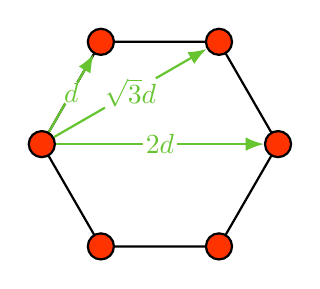
\begin{tikzpicture}[Benzene/.style={draw,thick, circle, radius = .1em,                                      fill=red!80!yellow},
                    arrow/.style={->, >=Latex,thick, yellow!40!green},
                    arrow_label/.style={midway, circle, fill=white, inner sep=0}
                    ]
        \newdimen\R
        \R=1.5cm
        \draw[thick] (0:\R)
        \foreach \x in {60,120,...,360} {  -- (\x:\R) }
        -- cycle (360:\R) node[Benzene] (Bc3){}
        -- cycle (300:\R) node[Benzene] (Bc4){}
        -- cycle (240:\R) node[Benzene] (Bc5){}
        -- cycle (180:\R) node[Benzene] (Bc0){}
        -- cycle (120:\R) node[Benzene] (Bc1){}
        -- cycle  (60:\R) node[Benzene] (Bc2){};
        
        \draw[arrow] (Bc0) -- (Bc1) node[arrow_label] {$d$};
        \draw[arrow] (Bc0) -- (Bc2) node[arrow_label] {$\sqrt{3}d$};
        \draw[arrow] (Bc0) -- (Bc3) node[arrow_label] {$2d$};
    \end{tikzpicture}
    \caption{Interatomic distances in Benzene ($d=\SI{1.40}{\angstrom})$}
    \label{fig:benzene_distances}
\end{figure}

\subsection{Hopping amplitudes}
One problem with modelling the benzene ring as a chain is that we lose the orientations of the bonds connecting neighbouring sites relative to the light pulse direction.
This leads to an inaccuracy in the angle-dependent time dependence of the hoppings between the sites, as illustrated in Fig. \ref{fig:benzene_angles}. However, by comparing the results with those of another group, where the orientation was taken into account, we saw only negligible differences in the results and thus choose to move forward with this model.
%\medskip
%lexicographical indexing no longer produces proper hopping signs... but as mentioned we ignore that for now
    %%%%%%%%%%%%%%%%%
    % PULSE ON LINE %
    %%%%%%%%%%%%%%%%%
    
\begin{figure}[!hbt]
    \centering
    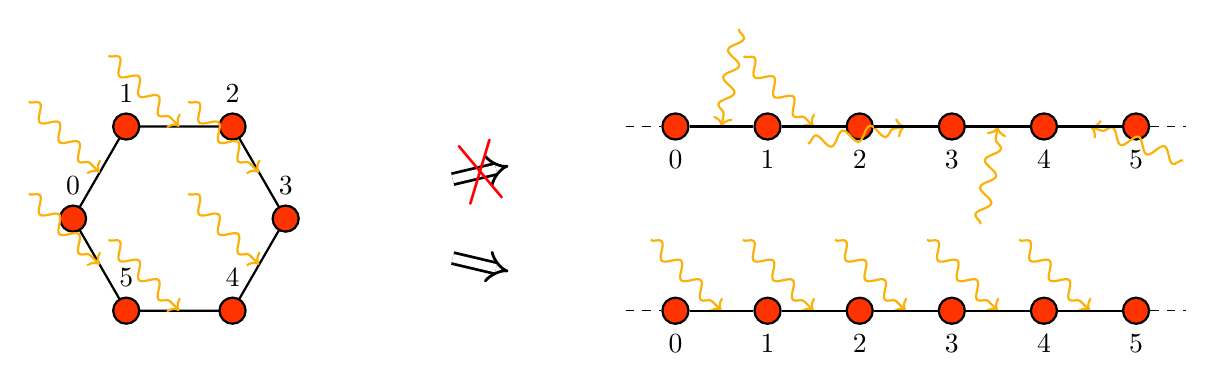
\begin{tikzpicture}[decoration=snake,
                    Benzene/.style={draw,thick, circle, radius = .1em, fill=red!80!yellow},
                    squiggly/.style={->, decorate, thick, yellow!70!red},
                    doublearrow/.style={->, double, line width=1pt, -Implies, double distance=3pt, shorten >= 2cm, shorten <=2cm},
                    scale=0.9
                    ]
                    
    
    % RING %
    \newdimen\R
    \R=1.5cm
    \draw[thick] (0:\R)
    \foreach \x in {60,120,...,360} {  -- (\x:\R) }
    -- cycle (360:\R) node[Benzene, label=3] (Bc3){}
    -- cycle (300:\R) node[Benzene, label=4] (Bc4){}
    -- cycle (240:\R) node[Benzene, label=5] (Bc5){}
    -- cycle (180:\R) node[Benzene, label=0] (Bc0){}
    -- cycle (120:\R) node[Benzene, label=1] (Bc1){}
    -- cycle  (60:\R) node[Benzene, label=2] (Bc2){};
    
    \foreach \x/\y in {0/1,1/2,2/3,3/4,4/5,5/0}{
    \draw[squiggly] ($(Bc\x)!0.5!(Bc\y) + (-1,1)$) -- ($(Bc\x)!0.5!(Bc\y)$);
    }
    
    
    % CHAIN DOWN%
    \foreach \x in {0,1,2,3,4,5}
    \node[Benzene, label=below:\x] at ($(1.3*\x,0) + (7,-1.3)$)  (B\x){};
    
    \foreach \x/\y in {0/1, 1/2, 2/3, 3/4, 4/5}
    \draw[squiggly] ($(B\x)!0.5!(B\y) + (-1, 1)$) -- ($(B\x)!0.5!(B\y)$);
    
    \foreach \x/\y in {0/1,1/2,2/3,3/4,4/5}
    \draw[thick] (B\x) -- (B\y);
    
    \draw[dashed] ($(B0) - (0.7,0)$) -- (B0);
    \draw[dashed] (B5) -- ($(B5) + (0.7,0)$);
    
    % CHAIN UP %
    \foreach \x in {0,1,2,3,4,5}
    \node[Benzene, label=below:\x] at ($(1.3*\x,0) + (7,1.3)$)  (Bu\x){};
    
    \foreach \x/\y/\angle in {0/1/80, 1/2/135, 2/3/190, 3/4/260, 4/5/340}
    \draw[squiggly] ($(Bu\x)!0.5!(Bu\y) + (\angle:1.4)$) -- ($(Bu\x)!0.5!(Bu\y)$);

    \foreach \x/\y in {0/1,1/2,2/3,3/4,4/5}
    \draw[thick] (Bu\x) -- (Bu\y);

    \draw[dashed] ($(Bu0) - (0.7,0)$) -- (Bu0);
    \draw[dashed] (Bu5) -- ($(Bu5) + (0.7,0)$);
    

    % DOUBLE ARROWS %
    \draw[doublearrow] (Bc3) -- (Bu0) node[pos=0.5,sloped,rotate=150]{\color{red}\Huge$|$}node[pos=0.5,rotate=40]{\color{red}\Huge$|$};
    \draw[doublearrow] (Bc3) -- (B0);
    \end{tikzpicture}
    \caption{Discrepancy in light pulse orientations relative to sites when modelling benzene as a 1D chain with periodic boundary conditions}
    \label{fig:benzene_angles}
\end{figure}
\newpage
\section{Coupling QD-Benzene}
\color{blue}
    The coupled QD-Benzene system is a combination of the above two systems with an extra hopping from all QD sites to a single Benzene site. Again the coulomb interactions are calculated via the Ohno interpolation and stored in the $U$ matrices. The distances used in the calculations for the $U$-matrix elements are shown in Fig. \ref{fig:coupled_distances}. The hopping amplitudes are the same as in the isolated systems with the addition of a parameter $v_c$, representing the hopping between the QD and the benzene ring. By setting $v_c = 0$ we would expect to see the same spectra as with the Isolated systems.{\color{red} at least for the QD, but for benzene idk because benzene not hit by laser pulse in this case... or is that irrelevant for the spectrum?}  Important to note: The on-site hoppings must be calculated individually for the Benzene and the QD sites. The hopping matrix is shown in Fig. \ref{fig:coupled_hoppings}
    \medskip
    
    For now we only investigate how the system responds to the light pulse only interacting with the QD sites. Thus we set all the benzene hoppings and the hoppings between the QD and benzene to be non-time dependent.
\color{black}

\begin{itemize}
    \item decided that investigate pulse only hitting quantum dot
    \item U matrices for couples systems
    \item equal and opposite spin matrices
    \item full coupling vs half coupling
    \item {\color{red} why would we expect to see impact ionisation in such a coupled system? previous papers?}
    \item separate $v_ii$ values for QD and Benzene
    \item why lehmann spectrum can not be computed and we need green
    \item hopping between QD and benzene NOT TIME DEPENDENT (pulse only on QD)
\end{itemize}

\usetikzlibrary{matrix, positioning}

\colorlet{mgreen}{green!80!black!30}
\colorlet{myellow}{yellow!90!red!70}
\newcommand{\my}{|[fill=myellow]|}
\renewcommand{\mg}{|[fill=mgreen]|}



\begin{figure}[!hbt]
    \centering
    \begin{tikzpicture}[cell/.style={rectangle,draw=black},
                    space/.style={minimum height=1.5em,matrix of nodes,row sep=-\pgflinewidth,column sep=-\pgflinewidth},
                    text depth=0.5ex,text height=2ex,nodes in empty cells,
                    headers/.style={font=\footnotesize, color=blue!60!black!30},
                    QD/.style={draw,thick,circle, radius = .1em, fill=black!40, inner sep=0},
                    Benzene/.style={draw,thick, circle, radius = .1em, fill=red!80!yellow, inner sep=0},
                    nlabelcolor/.style={gray},
                    QDlabel/.style={label={above left:{\color{gray}#1}}}
                    ]
    
    %maybe use brace to indicate Benzene and QD regions https://texample.net/tikz/examples/model-physics/
    \matrix (first) [space,nodes={cell,minimum width=2em, minimum height=2em}]
    {
    \my         & 1             & 1         & $\sqrt{2}$& \mg -     & -         & -         & -         & -         & -        \\
    1           & \my           & $\sqrt{2}$& 1         & \mg -     & -         & -         & -         & -         & -        \\
    1           & $\sqrt{2}$    & \my       & 1         & \mg -     & -         & -         & -         & -         & -        \\
    $\sqrt{2}$  & 1             & 1         & \my       & \mg -     & -         & -         & -         & -         & -        \\
    \mg -       & \mg -         & \mg -     & \mg -     & \my       & 1         & $\sqrt{3}$& 2         & $\sqrt{3}$& 1        \\
    -           & -             & -         & -        & 1         &  \my      & 1         & $\sqrt{3}$& 2         & $\sqrt{3}$ \\
    -           & -             & -         & -         & $\sqrt{3}$& 1         & \my       & 1         & $\sqrt{3}$& 2        \\
    -           & -             & -         & -         & 2         & $\sqrt{3}$& 1         &  \my      & 1         & $\sqrt{3}$ \\
    -           & -             & -         & -         & $\sqrt{3}$& 2         & $\sqrt{3}$& 1         & \my       & 1        \\
    -           & -             & -         & -         & 1         & $\sqrt{3}$& 2         & $\sqrt{3}$& 1         &  \my \\ };
    
    \foreach \i/\x in {0/1, 1/2,2/3,3/4,4/5,5/6, 6/7, 7/8, 8/9, 9/10}{
    \node[headers, anchor=north] at ([yshift=4ex]first-1-\x.north) {\i};
    \node[headers, anchor=west] at ([xshift=-4ex]first-\x-1.west) {\i};
    }
    %%%%%%%%%%%%%%%%%%%%%%%%%%%%%%%%%%%%%%%%%%%
    %%%%%%%%%%%%%%%%%%%%%%%%%%%%%%%%%%%%%%%%%%%
    \tikzset{shift={(6,1)}}
    \newdimen \qdd
    \qdd = 2cm
    %QD nodes    
    \node[QD, QDlabel={2}] at (0,0)          (QD2){};
    \node[QD, QDlabel={3}] at (\qdd,0)       (QD3){};
    \node[QD, QDlabel={0}] at (0,\qdd)       (QD0){};
    \node[QD, QDlabel={1}] at (\qdd,\qdd)    (QD1){};
    
    \draw[thick] (QD2.east) -- (QD3.west);
    \draw[thick] (QD0.east) -- (QD1.west);
    \draw[thick] (QD0.south) -- (QD2.north);
    \draw[thick] (QD1.south) -- (QD3.north);
    
    
    %Benzene Nodes
    \newdimen\R
    \R=1.5cm
    \tikzset{shift={(5,1)}}
    \draw[thick] (0:\R)
    \foreach \x in {60,120,...,360} {  -- (\x:\R) }
    -- cycle (360:\R) node[Benzene, label={[nlabelcolor]7}] (B7){}
    -- cycle (300:\R) node[Benzene, label={[nlabelcolor]8}] (B8){}
    -- cycle (240:\R) node[Benzene, label={[nlabelcolor]9}] (B9){}
    -- cycle (180:\R) node[Benzene, label={[nlabelcolor]4}] (B4){}
    -- cycle (120:\R) node[Benzene, label={[nlabelcolor]5}] (B5){}
    -- cycle  (60:\R) node[Benzene, label={[nlabelcolor]6}] (B6){};
    
    
    \tikzset{shift={(0,0)}}
    \foreach \x in {3, 1} \draw[color=red, thick] (QD\x.east) to [out=0, in=180] (B4.west);
    \draw[color=red, thick] (QD2.south) to [out = 270, in=180] (B4.west);
    \draw[color=red, thick] (QD0.north) to [out = 90, in=180] (B4.west);
    
    
    %%%%%%%%%%%%%%%%%%%%%%%%%%%%%%
    %%%%%%%%%%%%%%%%%%%%%%%%%%%%%%%
    % LEGEND
    
    \node [draw, rectangle, fill=myellow, minimum size=1em, inner sep=0, label={[align=left, text width=170pt]right: $\begin{cases} - &\text{ for equal spin matrix} \\ 1 &\text{ for opposite spin matrix}\end{cases}$}] at ($(QD2) + (0, -1.6)$) {};
    
    \node [draw, rectangle, fill=mgreen, minimum size=1em, inner sep=0, label={[align=left, text width=170pt]right: We assume strong shielding between benzene and quantum dot $\Rightarrow$ no Coulomb interaction}] at ($(QD2) + (0, -3.)$) {-};
    
    
    \end{tikzpicture}
    \caption{Table shows distances between sites, as multiples of the C-C bond length ($d=\SI{1.40}{\angstrom}$)... values in table are only inputs into ohno function though {\color{red} idk maybe add functions on how to generate table... prbly not nescessary though}, Note: ``-" $= \infty$}
    \label{fig:coupled_distances}
\end{figure}


%%%%%%%%%%%%%%%%%%%%%%%%%%%%%%%
%%%%%%%%%%%%%%%%%%%%%%%%%%%%%%%

\newcommand{\viiQD}   {|[fill=green!59]| $v_{ii}^{\text{qd}}$}
\newcommand{\viiBZ}   {|[fill=green!40]| $v_{ii}^{\text{b}}$}
\newcommand{\vh}    {|[fill=red!30]| $v_h$}
\newcommand{\vv}    {|[fill=yellow!80!red!50]| $v_v$}
\newcommand{\vd}    {|[fill=pink!50]| $v_d$}
\newcommand{\vc}    {|[fill=cyan!80!blue!20]| $v_c$}

\begin{figure}[!hbt]
    \centering
    \begin{tikzpicture}[cell/.style={rectangle,draw=black},
                    space/.style={minimum height=1.5em,matrix of nodes,row sep=-\pgflinewidth,column sep=-\pgflinewidth},
                    text depth=0.5ex,text height=2ex,nodes in empty cells,
                    headers/.style={font=\footnotesize, color=blue!60!black!30},
                    QD/.style={draw,thick,circle, radius = .1em, fill=green!80!yellow, inner sep=0},
                    Benzene/.style={draw,thick, circle, radius = .1em, fill=red!80!yellow, inner sep=0},
                    nlabelcolor/.style={gray},
                    QDlabel/.style={label={above left:{\color{gray}#1}}}
                    ]

    \matrix (first) [space,nodes={cell,minimum width=2.3em, minimum height=2.3em}]
    {
    \viiQD  & \vh   & \vv   & \vd  & \vc  & 0    & 0    & 0    & 0    & 0    \\
    \vh     & \viiQD& \vd   & \vv  & \vc  & 0    & 0    & 0    & 0    & 0    \\
    \vv     & \vd   & \viiQD& \vh  & \vc  & 0    & 0    & 0    & 0    & 0    \\
    \vd     & \vv   & \vh   & \viiQD & \vc  & 0    & 0    & 0    & 0    & 0    \\
    \vc     & \vc   & \vc   & \vc  & \viiBZ & \vh  & 0    & 0    & 0    & \vh  \\
    0       & 0     & 0     & 0    & \vh  & \viiBZ & \vh  & 0    & 0    & 0    \\
    0       & 0     & 0     & 0    & 0    & \vh  & \viiBZ & \vh  & 0    & 0    \\
    0       & 0     & 0     & 0    & 0    & 0    & \vh  & \viiBZ & \vh  & 0    \\
    0       & 0     & 0     & 0    & 0    & 0    & 0    & \vh  & \viiBZ & \vh  \\
    0       & 0     & 0     & 0    & \vh  & 0    & 0    & 0    & \vh  & \viiBZ \\ };
    
    \foreach \i/\x in {0/1, 1/2,2/3,3/4,4/5,5/6, 6/7, 7/8, 8/9, 9/10}{
    \node[headers, anchor=north] at ([yshift=4ex]first-1-\x.north) {\i};
    \node[headers, anchor=west] at ([xshift=-4ex]first-\x-1.west) {\i};
    }
    \end{tikzpicture}
    \caption{Table shows distances between sites, as multiples of the C-C bond length ($d=\SI{1.40}{\angstrom}$) {\color{red} idk maybe add functions on how to generate table... prbly not nescessary though}}
    \label{fig:coupled_hoppings}
\end{figure}

%
\chapter{Results and Conclusion}
\section{Isolated Quantum Dot}
\subsection{Engineering the spectrum}\label{subsec:spectrum_engineering}

To encourage impact ionisation, we engineer the quantum dot to have 4 equally spaced energy levels. As shown in Fig. \ref{fig:qd_spectrum_delta} (and Fig \ref{fig:impact_ionisation}) this allows for an electron from the lower Hubbard band to be excited into the most energetic state and during its subsequent decay, to promote a second electron over the Mott gap.
\newline
%{\color{red} do the lines represent states of electrons or states of the entire system?}

\begin{figure}[!hbt]
    \centering
    \begin{tikzpicture}[eline/.style={ultra thick, black},
                        earrow/.style={->, >=Latex, thick, shorten >=3pt, shorten <=3pt},
                        squiggly/.style={->, thick, decorate, decoration=snake, yellow!70!red}
                        ]
        
     
        \newdimen\height
        \height = 2.5cm
        \newdimen\baselength
        \baselength = 4cm
        \newdimen\arrowgap
        \arrowgap = 0.25cm
        
         % draw E axis and make nodes for energy levels
        \draw[->,>=stealth, ultra thick, black!50] ($(-\baselength,0)/2$) -- ($(\baselength,0)/2$) 
                                                    node[pos=0.5, inner sep=0, label=below:{\tiny E$_{\mathrm F}$}] (EF){}
                                                    node[pos=0.2, inner sep=0] (E1){}
                                                    node[pos=0.4, inner sep=0] (E2){}
                                                    node[pos=0.6, inner sep=0] (E3){}
                                                    node[pos=0.8, inner sep=0] (E4){}
                                                    node[pos=1, anchor=north]{\small E};
                                                            
        % tick for fermi energy
        \draw[thick, black!50] ($(EF) + (0,-3pt)$) -- ($(EF) + (0,3pt)$);
        
        % energy lines
        \foreach \i in {1, 2, 3, 4} 
        \draw[eline] (E\i) -- ($(E\i)+(0,\height)$) node[pos=0.5, inner sep=0] (halfE\i){};
        
        % electron transition lines
        % 1st arrow
        \draw[earrow, red]     ($(halfE2.west)+(0,\arrowgap)$) to [out = 30, in=150] 
                                node[pos=0.8, inner sep=1pt, outer sep=4pt, anchor=south, circle, draw]{\tiny$1$}
                                ($(halfE4.east)+(0,\arrowgap)$);
                                
        % impact io arrows
        \draw[earrow, black!60]     ($(halfE2.west)-(0,\arrowgap)$) to [out = 30, in= 150]  
                                node[pos=0.5, inner sep=0] (halfE23) {} 
                                ($(halfE3.east)-(0,\arrowgap)$);
                                
        \draw[earrow, black!60]     ($(halfE4.east)-(0,\arrowgap)$) to [out =-150, in=-30]  
                                node[pos=0.5, inner sep=0] (halfE43) {} 
                                node[pos=0.7, inner sep=1pt, outer sep=4pt, anchor=south, circle, draw]{\tiny$2$}
                                ($(halfE3.west)-(0,\arrowgap)$);
                               
        
        % squiggly line
        \draw[squiggly] (halfE43) to[out=-120, in=-80] (halfE23);
        
    \end{tikzpicture}
    \captionsetup{singlelinecheck=off}
    \caption{Illustration of why equally spaced energy levels encourage impact ionisation through Coulomb interactions.
    \newline
    1. An electron is promoted by two energy levels. 
    \newline
    2. The promoted electron gives up half its energy to promote a second electron (squiggly line)}
    \label{fig:qd_spectrum_delta}
\end{figure}

The main parameter that needs to be tuned to achieve such a spectrum is the on site coulomb potential $U \equiv U_{ii}$, as it is directly responsible for the size of the Mott gap. A loop was set up to compute the Lehmann spectrum of the system for a range of values of $U$. The mean differences in the spacings between the peaks were extracted and plotted as a function of the coulomb potential. By regressing a line to this data we were then able to determine that for our choice of parameters, $U = 2.41$ produced the desired energy level spacing. Fig. \ref{fig:spectrum_engineering} shows a series of Lehmann spectra that were produced in this process as well as the final, equally spaced spectrum.


\begin{figure}[!hbt]
    \centering
    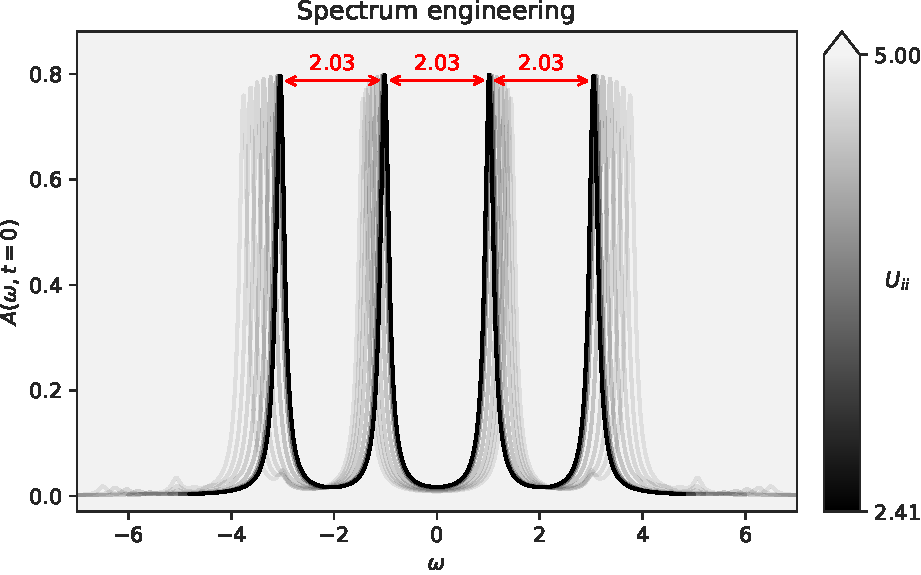
\includegraphics[width=0.7\textwidth]{graph/spectrum_engineering.pdf}
    \caption{Equilibrium spectral function $A(\omega)$ on site 0.}
    \label{fig:spectrum_engineering}
\end{figure}

\subsection{Why the spectral function may not be a good choice for small systems}
In Fig. \ref{fig:qd_9_total_energy} we see the total energy of the spectrum engineered QD over time, after being subjected to a light pulse of varying frequencies $\omega$. As expected, for low values of $\omega$ no electrons can be excited over the Mott gap and thus no energy from the light pulse is absorbed. At $\omega = 2.00$ (\color{red} units of t?\color{black}) we see an energy increase as the light is now energetic enough to promote an electron into the upper hubbard band.

\medskip

Rather unexpectedly however, we see no energy gain at $\omega = 4.00$, meaning the first transition shown in Fig. \ref{fig:qd_spectrum_delta} seems to not be taking place.

\medskip

One possible explanation for this may be that the spectral functions we are using are not truly representative of the transitions between the eigenstates of our system. As briefly explained in section \ref{sec:spectral_functions}, we compute spectral functions by adding an electron/hole to the system, letting it propagate for a fixed time, then removing it again, and evaluating the overlap of this system with an unmodified one. Thus the spectral function shows us transitions between systems with electron numbers differing by one. For large systems, with many electrons, adding or removing a single electron has an insignificant effect on its eigenenergy spectrum and thus it will be equal to the spectral function. However, for a small 2x2 site system like our QD, the effect may no longer be negligible. Meaning that the one-particle spectrum we see in Fig. \ref{fig:spectrum_engineering} may not accurately represent the optical transitions possible in the QD.

\medskip
It may be possible to remedy this with the use of Loschmid spectra, which do not suffer from the same issues in small systems \cite{loschmidt}. However the implementation of these will have to wait for a future work. 

\medskip

\begin{figure}[!hbt]
    \centering
    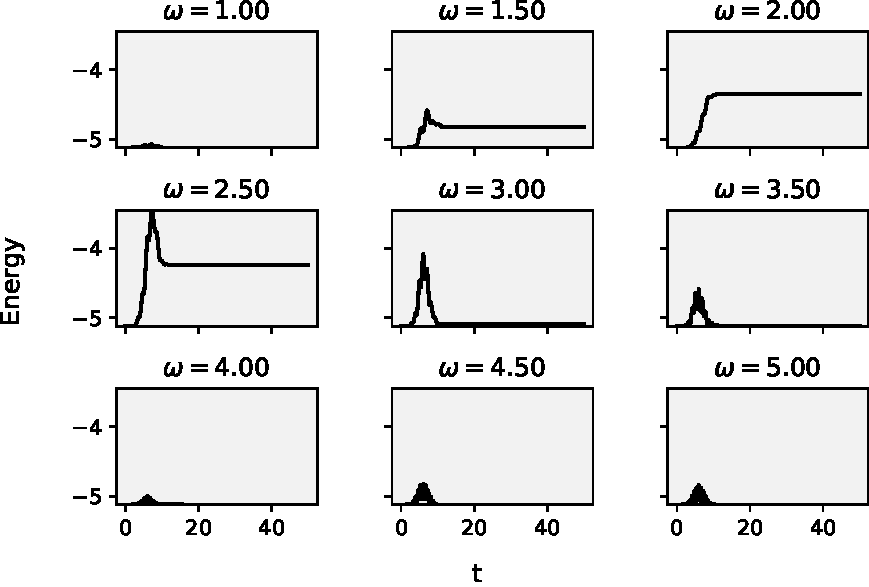
\includegraphics[width=0.7\textwidth]{graph/9test.pdf}
    \caption{Total energy in isolated QD system after interaction with light pulse at $t=6$ for various frequencies $\omega$.}
    \label{fig:qd_9_total_energy}
\end{figure}
\section{Isolated Benzene}

\begin{figure}[!hbt]
    \centering
    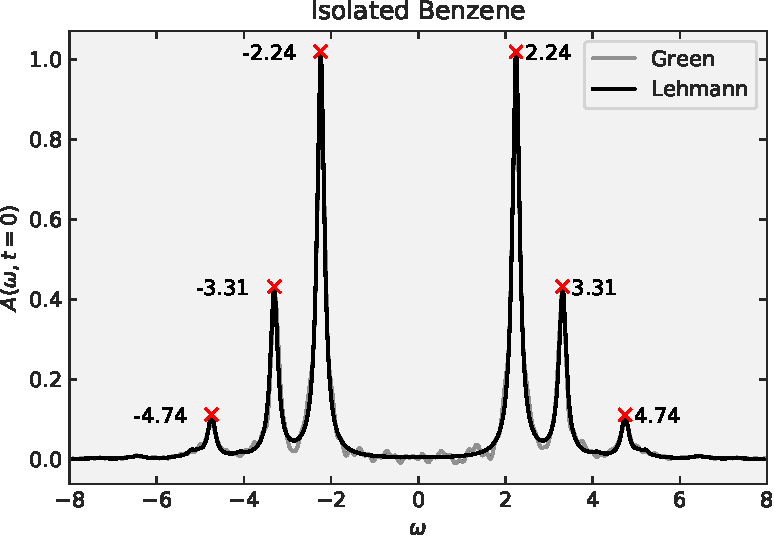
\includegraphics[width=0.7\textwidth]{graph/isolated_benzene.pdf}
    \caption{temporary. also have nonequilibrium plots. But are those interesting? Do not see much change. maybe need to look at time dependence of hoppings again}
\end{figure}

\section{Coupled System}

\subsection{Testing}
Before we investigate the effects of increasing the coupling strength between the two systems, we verify that if the hopping amplitude $v_c = 0$, the spectra on the individual sites remain unchanged. For the coupled system, calculating the Lehmann spectrum is no longer an option as memory becomes a limiting factor, instead we resort to using the Green's function method.

\medskip
As can be seen when comparing Fig. \ref{fig:coupled_vc_0} with the spectra in Fig. \ref{fig:spectrum_engineering} and Fig. \ref{fig:isolated_benzene}, this is indeed the case. The slight variations being due to a difference in parameters used to perform the Fourier transformation.

\begin{figure}[!hbt]
    \centering
    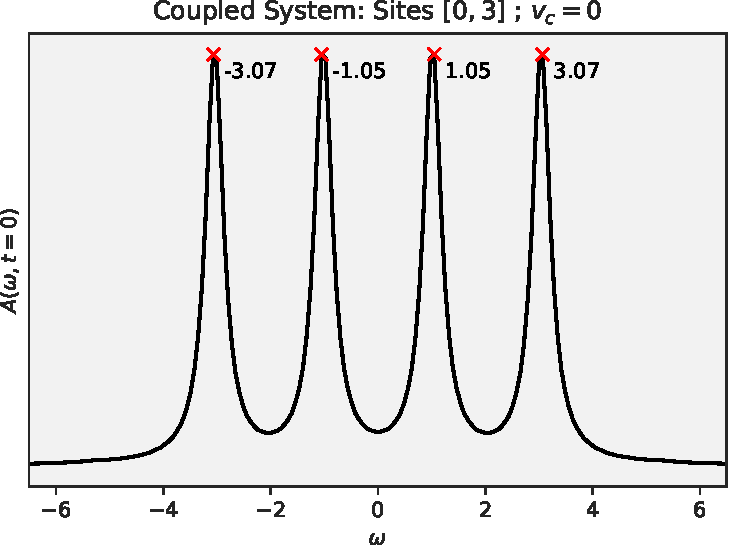
\includegraphics[width=0.49\textwidth]{graph/coupled_QD_vc_0.pdf}
    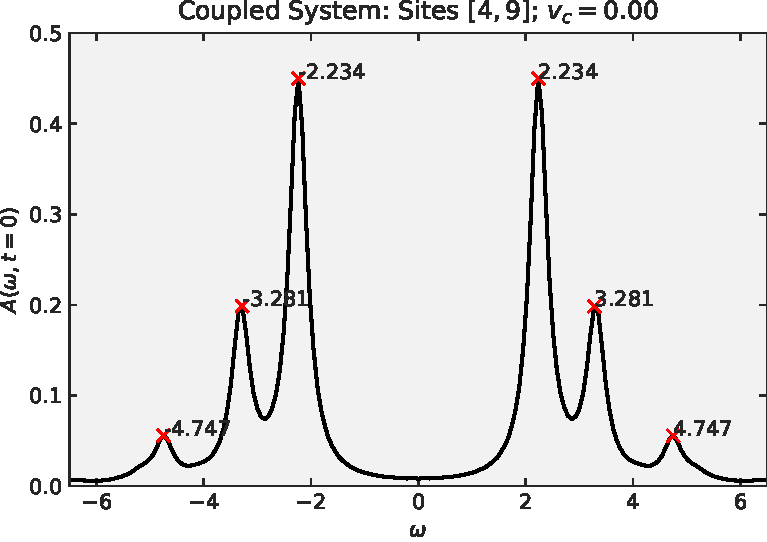
\includegraphics[width=0.49\textwidth]{graph/coupled_benzene_vc_0.pdf}sh
    \caption{Spectral function of all the sites of the coupled system with the coupling parameter turned off, $v_c = 0$. These spectra should be identical to those in Fig. \ref{fig:spectrum_engineering} and Fig. \ref{fig:isolated_benzene}}
    \label{fig:coupled_vc_0}
\end{figure}

\subsection{Dependence of the spectrum on the coupling strength}

\begin{figure}[!hbt]
    \centering
    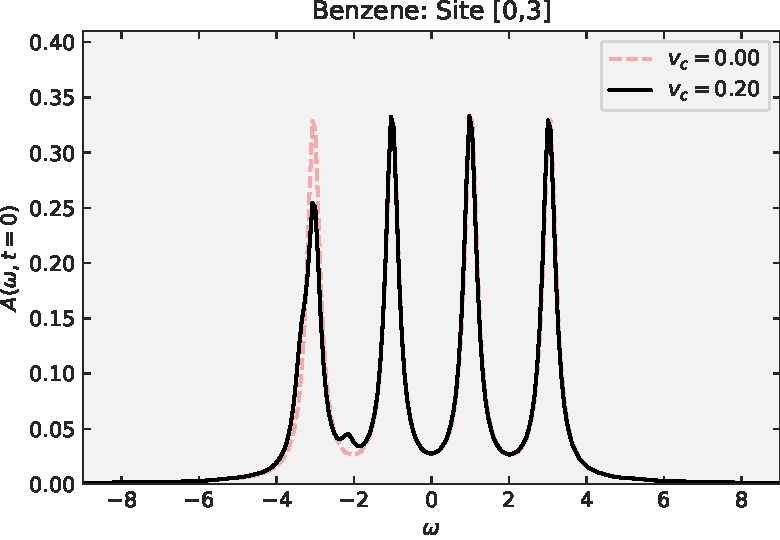
\includegraphics[width=0.49\textwidth]{graph/spectrum_vc_sweep/QD_All_020.pdf}
    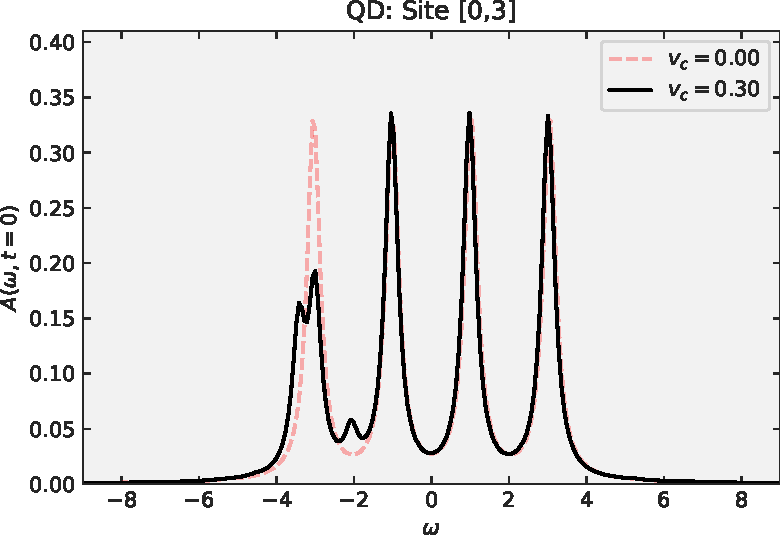
\includegraphics[width=0.49\textwidth]{graph/spectrum_vc_sweep/QD_All_030.pdf}
    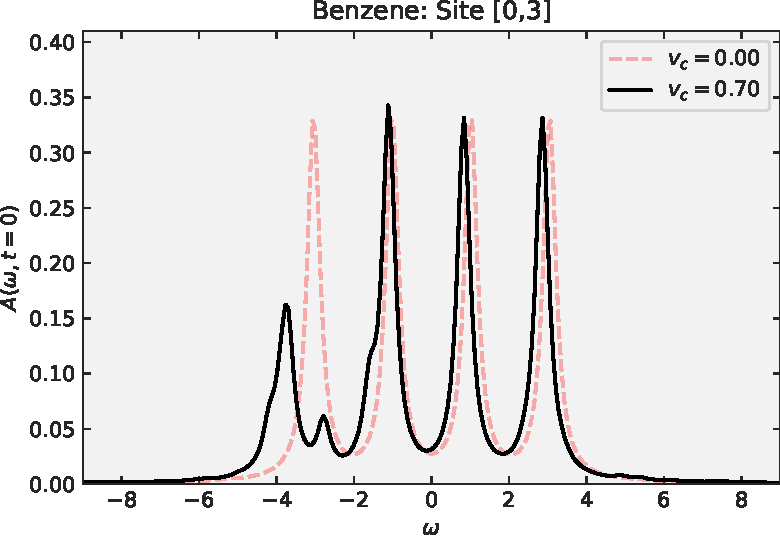
\includegraphics[width=0.49\textwidth]{graph/spectrum_vc_sweep/QD_All_070.pdf}
    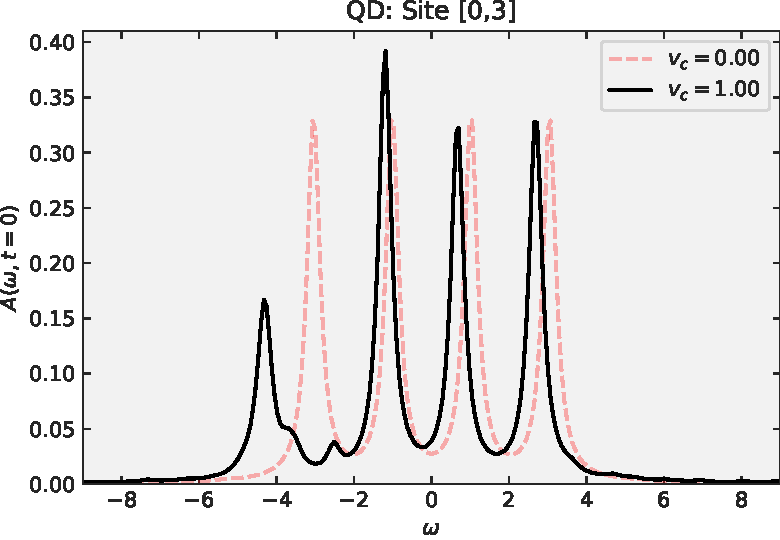
\includegraphics[width=0.49\textwidth]{graph/spectrum_vc_sweep/QD_All_100.pdf}
    \caption{}
    \label{fig:spectrum_vc_sweep}
\end{figure}
\newpage

%  1. Introduction to this topic
%     - keep it short (1-2pages)
%     - reference Hörbinger + original PPP papers
%     - Innerberger
    
%  2. Code that I implemented
%     - non-local interaction
%     - potential energy (instead of double occupancy)... double occupancy not a good measure of pot energy anymore
%     - vii (Hubbard term)

% 3. Results
%     - Greens functions
%     - show QD and Benzene isolated (compare to PPP paper)
%     - show coupled QD and Benzene (with vc = 0 and with vc != 0)
    
% 4. Outlook
%     - this was about the setup
%     - next work is about analysing this system (impact ionisation on BzRing or QD)
%     - why no transitions as w=4 (maybe some k point stuff)
    
% What the reader should get from the thesis
% 1.(How the new implemented code works and how one can use it)
% 2.(How does a spectrum of QD to Benzene ring look)

%\newpage
%\chapter*{Parameters for figures}
%Maybe explain parameter shorthands here {\color{red} All values are placeholders for now}

\begin{table}[!hbt]
\centering
    \begin{tabular}{SSSSSSSSSSS} \toprule
        {Fig.} & {U} & {w} & {a} & {vd} & {vc} & {s} & {Tend} & {deltaT} & {eps} \\ \midrule
        0.00  & 0.00 & 0.00 & 0.00 & 0.00 & 0.00 & 0.00 & 0.00 & 0.00 & 0.00 & 0.00\\
        0.00  & 0.00 & 0.00 & 0.00 & 0.00 & 0.00 & 0.00 & 0.00 & 0.00 & 0.00 & 0.00\\
        0.00  & 0.00 & 0.00 & 0.00 & 0.00 & 0.00 & 0.00 & 0.00 & 0.00 & 0.00 & 0.00\\
        0.00  & 0.00 & 0.00 & 0.00 & 0.00 & 0.00 & 0.00 & 0.00 & 0.00 & 0.00 & 0.00\\
        0.00  & 0.00 & 0.00 & 0.00 & 0.00 & 0.00 & 0.00 & 0.00 & 0.00 & 0.00 & 0.00\\
        0.00  & 0.00 & 0.00 & 0.00 & 0.00 & 0.00 & 0.00 & 0.00 & 0.00 & 0.00 & 0.00\\
        0.00  & 0.00 & 0.00 & 0.00 & 0.00 & 0.00 & 0.00 & 0.00 & 0.00 & 0.00 & 0.00\\
    \end{tabular}
    \caption{Table showing parameters used to compute figures (placeholder data for now)}
    \label{tab:data_table}
\end{table}
\newpage


\addcontentsline{toc}{chapter}{Bibliographie} % add to table of content without needing an actual heading
\bibliographystyle{unsrt} % https://www.overleaf.com/learn/latex/Bibtex_bibliography_styles
\bibliography{other/bibliography.bib} 

%\newpage
%% diagram idea https://texample.net/tikz/examples/tcp-state-machine/

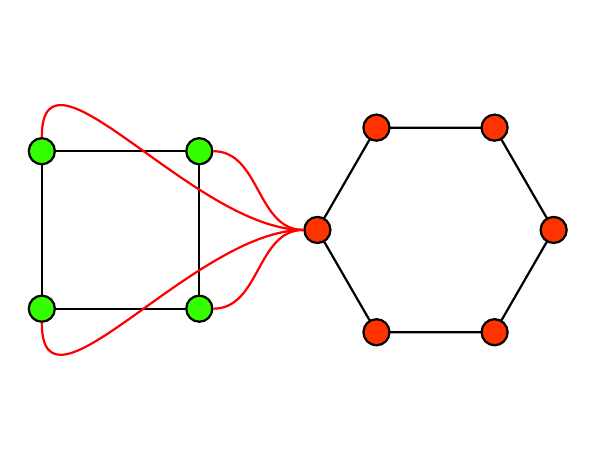
\begin{tikzpicture}[%
    QD/.style={draw,thick,circle, radius = .1em, fill=green!80!yellow},
    Benzene/.style={draw,thick, circle, radius = .1em, fill=red!80!yellow}
    ]
    
    \newdimen \qdd
    \qdd = 2cm
    %QD nodes    
    \node[QD] at (0,0)          (QD0){};
    \node[QD] at (\qdd,0)       (QD1){};
    \node[QD] at (0,\qdd)       (QD2){};
    \node[QD] at (\qdd,\qdd)    (QD3){};
    
    \draw[thick] (QD0.east) -- (QD1.west);
    \draw[thick] (QD2.east) -- (QD3.west);
    \draw[thick] (QD2.south) -- (QD0.north);
    \draw[thick] (QD3.south) -- (QD1.north);
    
    
    %Benzene Nodes
    \newdimen\R
    \R=1.5cm
    \tikzset{shift={(5,1)}}
    \draw[thick] (0:\R)
    \foreach \x in {60,120,...,360} {  -- (\x:\R) }
    -- cycle (360:\R) node[Benzene] (B0){}
    -- cycle (300:\R) node[Benzene] (B1){}
    -- cycle (240:\R) node[Benzene] (B2){}
    -- cycle (180:\R) node[Benzene] (B3){}
    -- cycle (120:\R) node[Benzene] (B4){}
    -- cycle  (60:\R) node[Benzene] (B5){};
    
    \tikzset{shift={(0,0)}}
    \foreach \x in {1, 3} \draw[color=red, thick] (QD\x.east) to [out=0, in=180] (B3.west);
    \draw[color=red, thick] (QD0.south) to [out = 270, in=180] (B3.west);
    \draw[color=red, thick] (QD2.north) to [out = 90, in=180] (B3.west);
\end{tikzpicture}

\vskip 5cm
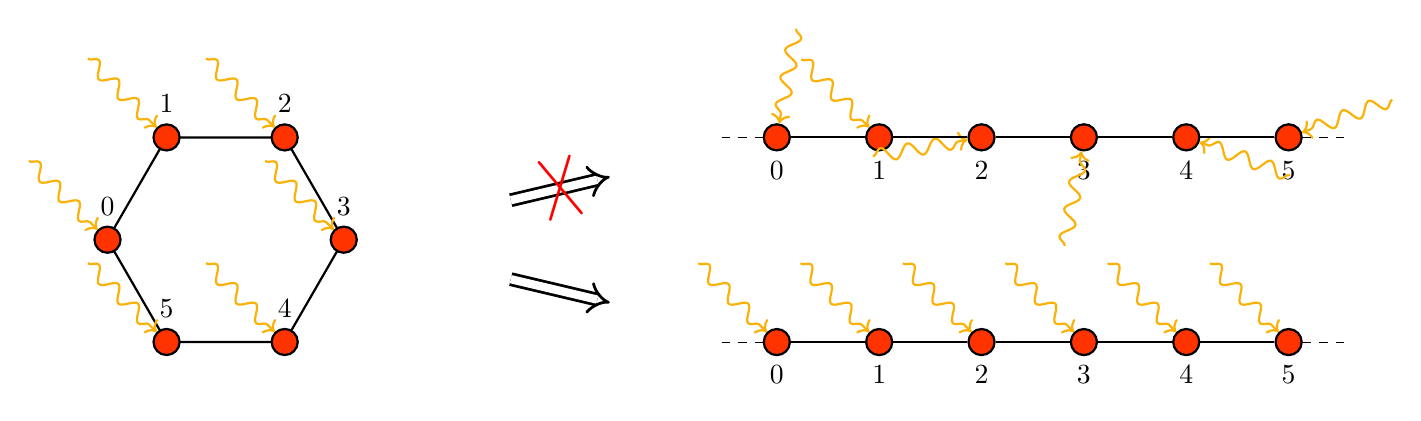
\begin{tikzpicture}[decoration=snake,
                    Benzene/.style={draw,thick, circle, radius = .1em, fill=red!80!yellow},
                    squiggly/.style={->, decorate, thick, yellow!70!red},
                    doublearrow/.style={->, double, line width=1pt, -Implies, double distance=3pt, shorten >= 2cm, shorten <=2cm}
                    ]
    % RING %
    \newdimen\R
    \R=1.5cm
    \draw[thick] (0:\R)
    \foreach \x in {60,120,...,360} {  -- (\x:\R) }
    -- cycle (360:\R) node[Benzene, label=3] (Bc3){}
    -- cycle (300:\R) node[Benzene, label=4] (Bc4){}
    -- cycle (240:\R) node[Benzene, label=5] (Bc5){}
    -- cycle (180:\R) node[Benzene, label=0] (Bc0){}
    -- cycle (120:\R) node[Benzene, label=1] (Bc1){}
-- cycle  (60:\R) node[Benzene, label=2] (Bc2){};
    
    \foreach \x in {0,1,2,3,4,5}{
    \draw[squiggly] ($(Bc\x) + (-1, 1)$) -- (Bc\x);
    }
    
    % CHAIN DOWN%
    \foreach \x in {0,1,2,3,4,5}{
    \node[Benzene, label=below:\x] at ($(1.3*\x,0) + (7,-1.3)$)  (B\x){};
    \draw[squiggly] ($(B\x) + (-1, 1)$) -- (B\x);
    }

    \foreach \x/\y in {0/1,1/2,2/3,3/4,4/5}{
    \draw[thick] (B\x) -- (B\y);
    }
    \draw[dashed] ($(B0) - (0.7,0)$) -- (B0);
    \draw[dashed] (B5) -- ($(B5) + (0.7,0)$);
    
    % CHAIN UP %
    \foreach \x in {0,1,2,3,4,5}
    \node[Benzene, label=below:\x] at ($(1.3*\x,0) + (7,1.3)$)  (Bu\x){};
    
    \foreach \x/\angle in {0/80, 1/135, 2/190, 3/260, 4/340, 5/20}
    \draw[squiggly] ($(Bu\x) + (\angle:1.4)$) -- (Bu\x);
    
    \foreach \x/\y in {0/1,1/2,2/3,3/4,4/5}
    \draw[thick] (Bu\x) -- (Bu\y);
    
    \draw[dashed] ($(Bu0) - (0.7,0)$) -- (Bu0);
    \draw[dashed] (Bu5) -- ($(Bu5) + (0.7,0)$);
    
    % DOUBLE ARROWS %
    \draw[doublearrow] (Bc3) -- (Bu0) node[pos=0.5,sloped,rotate=150]{\color{red}\Huge$|$}node[pos=0.5,rotate=40]{\color{red}\Huge$|$};
    \draw[doublearrow] (Bc3) -- (B0);
    
\end{tikzpicture}

\end{document}